% Created 2023-02-05 dom 21:44
% Intended LaTeX compiler: pdflatex
\documentclass[aspectratio=169, usenames,svgnames,dvipsnames]{beamer}
\usepackage[utf8]{inputenc}
\usepackage[T1]{fontenc}
\usepackage{graphicx}
\usepackage{longtable}
\usepackage{wrapfig}
\usepackage{rotating}
\usepackage[normalem]{ulem}
\usepackage{amsmath}
\usepackage{amssymb}
\usepackage{capt-of}
\usepackage{hyperref}
\usepackage{color}
\usepackage{listings}
\usepackage{mathpazo}
\usepackage{gensymb}
\usepackage{amsmath}
\usepackage{diffcoeff}
\usepackage{steinmetz}
\usepackage{mathtools}
\bibliographystyle{plain}
\usepackage{siunitx}
\sisetup{output-decimal-marker={,}}
\DeclareSIUnit{\watthour}{Wh}
\hypersetup{colorlinks=true, linkcolor=Blue, urlcolor=Blue}
\renewcommand{\thefootnote}{\fnsymbol{footnote}}
\newcommand{\laplace}[1]{\mathbf{#1}(\mathbf{s})}
\newcommand{\slp}{\mathbf{s}}
\newcommand{\fasor}[1]{\mathbf{#1}(\omega)}
\newcommand{\atan}{\mathrm{atan}}
\parskip=5pt
\usetheme{Boadilla}
\usecolortheme{rose}
\usefonttheme{serif}
\author{Oscar Perpiñán Lamigueiro}
\date{}
\title{Elementos Activos}
\subtitle{Teoría de Circuitos II}
\setbeamercolor{alerted text}{fg=blue!50!black} \setbeamerfont{alerted text}{series=\bfseries}
\AtBeginSubsection[]{\begin{frame}[plain]\tableofcontents[currentsubsection,sectionstyle=show/shaded,subsectionstyle=show/shaded/hide]\end{frame}}
\AtBeginSection[]{\begin{frame}[plain]\tableofcontents[currentsection,hideallsubsections]\end{frame}}
\beamertemplatenavigationsymbolsempty
\setbeamertemplate{footline}[frame number]
\setbeamertemplate{itemize items}[triangle]
\setbeamertemplate{enumerate items}[circle]
\setbeamertemplate{section in toc}[circle]
\setbeamertemplate{subsection in toc}[circle]
\hypersetup{
 pdfauthor={Oscar Perpiñán Lamigueiro},
 pdftitle={Elementos Activos},
 pdfkeywords={},
 pdfsubject={},
 pdfcreator={Emacs 28.2 (Org mode 9.6)}, 
 pdflang={Spanish}}
\begin{document}

\maketitle

\section{Clasificación}
\label{sec:org01f5bbd}
\begin{frame}[label={sec:org0beeadc}]{Clasificación}
\begin{itemize}
\item Tensión o Corriente
\item Ideal o Real
\item Dependiente o Independiente
\end{itemize}
\end{frame}

\begin{frame}[label={sec:orga11000a}]{Generador Ideal}
\begin{columns}
\begin{column}{0.5\columnwidth}
\begin{center}
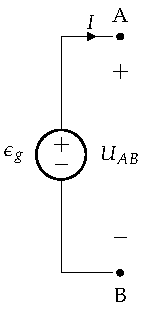
\includegraphics[height=0.5\textheight]{../figs/FuenteTensionIdealDC.pdf}
\end{center}
Un \alert{generador de tensión ideal} impone la tensión a la salida (\emph{la corriente depende del circuito}). Se caracteriza por su \alert{fuerza electromotriz} (voltios [V]).
\end{column}

\begin{column}{0.5\columnwidth}
\begin{center}
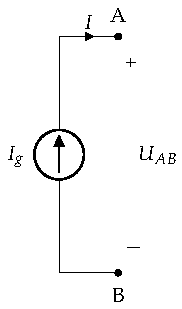
\includegraphics[height=0.5\textheight]{../figs/FuenteCorrienteIdeal.pdf}
\end{center}
Un \alert{generador de corriente ideal} impone la corriente a la salida (\emph{la tensión depende del circuito}). Se caracteriza por su corriente de generador.
\end{column}
\end{columns}
\end{frame}

\begin{frame}[label={sec:org5a0e35c}]{Generador Real CC}
Los generadores reales tienen pérdidas que se modelan con una resistencia en \alert{serie} (generador de tensión) o en \alert{paralelo} (generador de corriente)

\begin{columns}
\begin{column}{0.5\columnwidth}
\begin{center}
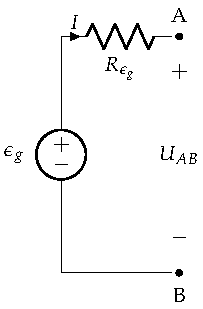
\includegraphics[height=0.7\textheight]{../figs/FuenteTensionRealDC.pdf}
\end{center}
\end{column}
\begin{column}{0.5\columnwidth}
\begin{center}
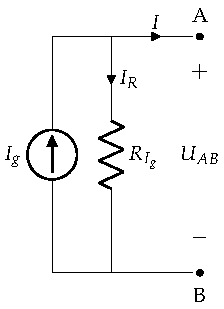
\includegraphics[height=0.7\textheight]{../figs/FuenteCorrienteRealDC.pdf}
\end{center}
\end{column}
\end{columns}
\end{frame}

\begin{frame}[label={sec:org62fa2f4}]{Generador Real AC}
Los generadores reales tienen pérdidas que se modelan con una impedancia en \alert{serie} (generador de tensión) o en \alert{paralelo} (generador de corriente)

\begin{columns}
\begin{column}{0.5\columnwidth}
\begin{center}
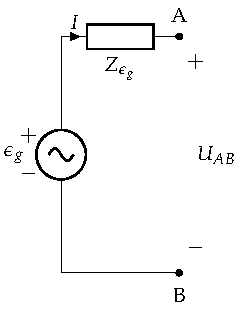
\includegraphics[height=0.5\textheight]{../figs/FuenteTensionReal.pdf}
\end{center}
\[
  \overline{U}_{AB} = \overline{\epsilon}_g - \overline{Z}_{\epsilon_g} \cdot \overline{I}
\]
\end{column}
\begin{column}{0.5\columnwidth}
\begin{center}
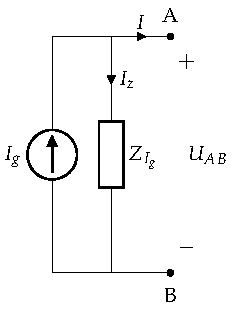
\includegraphics[height=0.5\textheight]{../figs/FuenteCorrienteReal.pdf}
\end{center}
\[
  \overline{I} = \overline{I}_g - \frac{\overline{U}_{AB}}{\overline{Z}_{I_g}}
\]
\end{column}
\end{columns}
\end{frame}


\begin{frame}[label={sec:org61e5888}]{Generadores Dependientes}
\begin{block}{Generadores de Tensión}
\begin{columns}
\begin{column}{0.5\columnwidth}
  \begin{center}
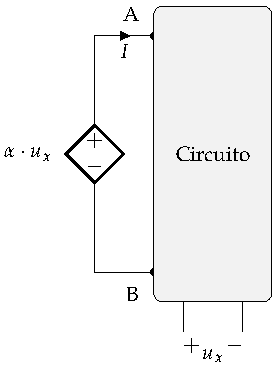
\includegraphics[height=0.7\textheight]{../figs/FuenteTensionDependienteTension.pdf}
\end{center}
\ldots{} de Tensión
\end{column}
\begin{column}{0.5\columnwidth}
  \begin{center}
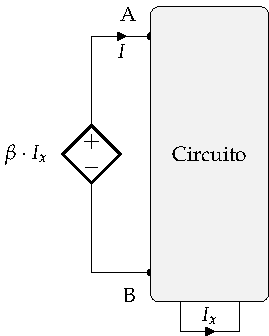
\includegraphics[height=0.7\textheight]{../figs/FuenteTensionDependienteCorriente.pdf}
\end{center}
\ldots{} de Corriente
\end{column}
\end{columns}
\end{block}
\end{frame}
\begin{frame}[label={sec:orge739451}]{Generadores Dependientes}
\begin{block}{Generadores de Corriente}
\begin{columns}
\begin{column}{0.5\columnwidth}
 \begin{center}
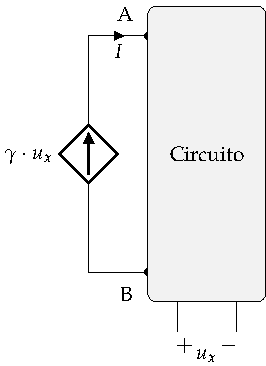
\includegraphics[height=0.7\textheight]{../figs/FuenteCorrienteDependienteTension.pdf}
\end{center}
\ldots{} de Tensión
\end{column}
\begin{column}{0.5\columnwidth}
 \begin{center}
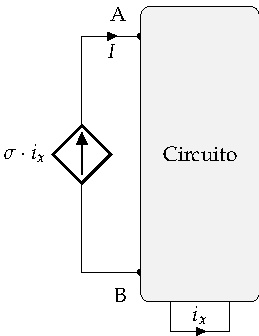
\includegraphics[height=0.7\textheight]{../figs/FuenteCorrienteDependienteCorriente.pdf}
\end{center}
\ldots{} de Corriente
\end{column}
\end{columns}
\end{block}
\end{frame}


\section{Generadores Independientes Reales}
\label{sec:org9a8c202}

\begin{frame}[label={sec:orgc1de786}]{Ecuación del generador CC}
\begin{columns}
\begin{column}{0.5\columnwidth}
\begin{center}
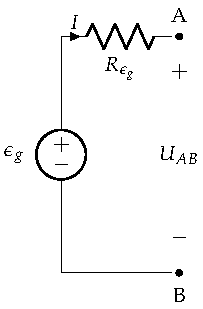
\includegraphics[height=0.5\textheight]{../figs/FuenteTensionRealDC.pdf}
\end{center}
\[
  U_{AB} = \epsilon_g - R_{\epsilon_g} \cdot I
\]
\end{column}
\begin{column}{0.5\columnwidth}
\begin{center}
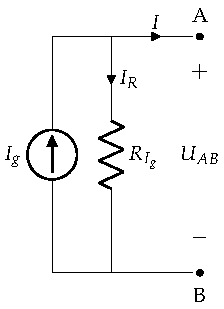
\includegraphics[height=0.5\textheight]{../figs/FuenteCorrienteRealDC.pdf}
\end{center}
\[
  I = I_g - \frac{U_{AB}}{R_{I_g}}
\]
\end{column}
\end{columns}
\end{frame}
\begin{frame}[label={sec:org38968fd}]{Ecuación del generador AC}
\begin{columns}
\begin{column}{0.5\columnwidth}
\begin{center}
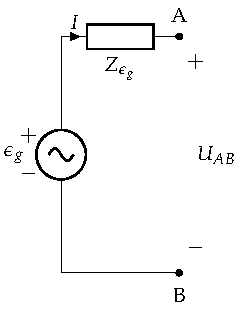
\includegraphics[height=0.5\textheight]{../figs/FuenteTensionReal.pdf}
\end{center}
\[
  \overline{U}_{AB} = \overline{\epsilon}_g - \overline{Z}_{\epsilon_g} \cdot \overline{I}
\]
\end{column}
\begin{column}{0.5\columnwidth}
\begin{center}
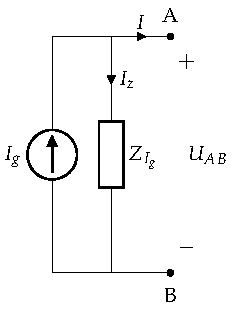
\includegraphics[height=0.5\textheight]{../figs/FuenteCorrienteReal.pdf}
\end{center}
\[
  \overline{I} = \overline{I}_g - \frac{\overline{U}_{AB}}{\overline{Z}_{I_g}}
\]
\end{column}
\end{columns}
\end{frame}

\begin{frame}[label={sec:org3dc572d}]{Diagramas Tensión - Corriente}
\begin{columns}
\begin{column}{0.5\columnwidth}
Fuente de tensión
\begin{center}
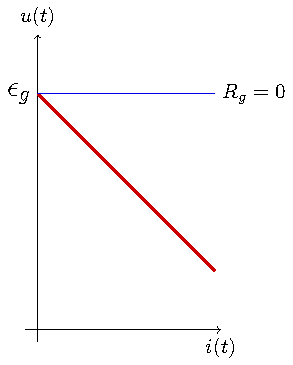
\includegraphics[height=0.5\textheight]{../figs/FuenteTension_DiagramaTensionCorriente.pdf}
\end{center}
\begin{align*}
  u(t) &= \epsilon_g - R_{\epsilon_g} \cdot i(t)\\
  i(t) &= 1/R_{\epsilon_g} \cdot (\epsilon_g - u(t))
\end{align*}
\end{column}
\begin{column}{0.5\columnwidth}
Fuente de corriente
\begin{center}
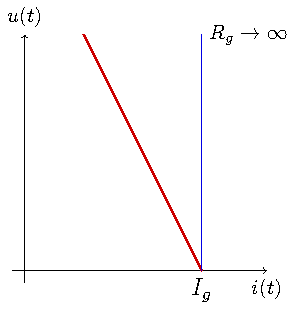
\includegraphics[height=0.5\textheight]{../figs/FuenteCorriente_DiagramaTensionCorriente.pdf}
\end{center}
\begin{align*}
  i(t) &= I_g - u(t)/R_{Ig}\\
  u(t) &= R_{Ig} \cdot (I_g - i(t))
\end{align*}
\end{column}
\end{columns}
\end{frame}
\begin{frame}[label={sec:org52da12a}]{Potencia y rendimiento de una fuente}
\begin{columns}
\begin{column}{0.4\columnwidth}
\begin{center}
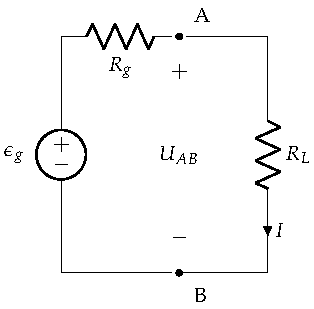
\includegraphics[height=0.55\textheight]{../figs/FuenteTensionRealConCarga.pdf}
\end{center}
\end{column}

\begin{column}{0.6\columnwidth}
\[
  \left.
    \begin{array}{c}
      I = \epsilon_g/(R_g + R_L)\\
      \\
      P_g = \epsilon_g \cdot I\\
      \\
      P_L = I^2 \cdot R_L
    \end{array} \right\}
  \rightarrow \left\{
    \begin{array}{c}
      P_g = \frac{\epsilon^2_g}{(R_g + R_L)}\\
      \\
      P_L = \frac{\epsilon^2_g \cdot R_L}{(R_g + R_L)^2}\\
      \\
      \eta = \frac{P_L}{P_g} = \frac{R_L}{R_g + R_L}
    \end{array}\right.
\]
\end{column}
\end{columns}
\end{frame}

\begin{frame}[label={sec:org92b5379}]{Potencia y rendimiento de una fuente}
\begin{columns}
\begin{column}{0.5\columnwidth}
\begin{itemize}
\item Suponiendo \(R_g\) constante, la potencia entregada por la fuente es máxima cuando \(R_L = R_g\).
\end{itemize}

\begin{equation*}
  P_L = \frac{\epsilon^2_{th}}{4 R_g}
\end{equation*}

\begin{itemize}
\item El rendimiento es una función creciente (\(\eta \to 1\) para \(R_L \gg R_g\)).
\end{itemize}
\end{column}

\begin{column}{0.5\columnwidth}
\begin{center}
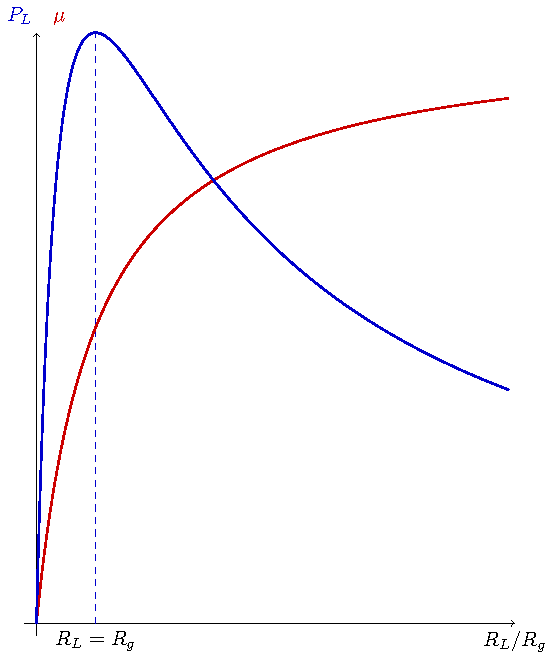
\includegraphics[height=0.85\textheight]{../figs/FuenteReal_PotenciaRendimiento.pdf}
\end{center}
\end{column}
\end{columns}
\end{frame}

\begin{frame}[label={sec:orgfa1cc5f}]{Potencia y rendimiento de una fuente}
\begin{columns}
\begin{column}{0.5\columnwidth}
\begin{itemize}
\item En la zona a la derecha del punto de máxima potencia (\(R_L > R_g\)), la función de potencia tiene una variación suave: los cambios en \(R_L\) tienen un impacto pequeño en \(P_L\).
\item Por ejemplo:
\begin{itemize}
\item Para \(R_L = R_g\) se obtiene \(\eta = 0'5\)
\item Para \(R_L = 2\cdot R_g\), se obtiene \(P_L = 0'89 \cdot P_{max}\) y \(\eta = 0'67\).
\item Para \(R_L = 3\cdot R_g\), se obtiene \(P_L = 0'75 \cdot P_{max}\) y \(\eta = 0'75\).
\end{itemize}
\end{itemize}
\end{column}
\begin{column}{0.5\columnwidth}
\begin{center}
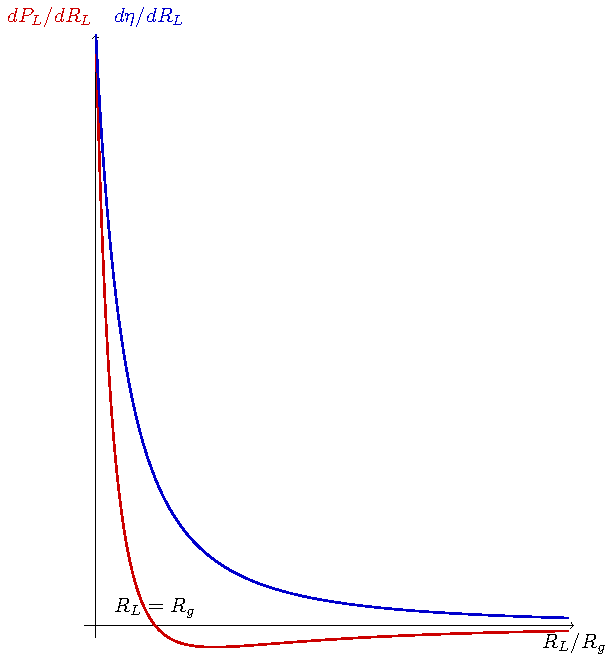
\includegraphics[height=0.85\textheight]{../figs/FuenteReal_DifPotencia.pdf}
\end{center}
\end{column}
\end{columns}
\end{frame}

\begin{frame}[label={sec:org53f444a}]{Potencia de una fuente AC}
Calculamos la potencia activa en la impedancia de carga \(Z_L\):
\begin{columns}
\begin{column}{0.3\columnwidth}
\begin{center}
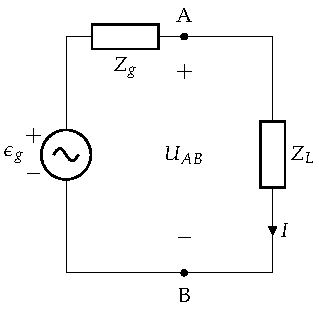
\includegraphics[height=0.45\textheight]{../figs/FuenteTensionRealACConCarga.pdf}
\end{center}
\end{column}

\begin{column}{0.2\columnwidth}
\begin{align*}
  \overline{Z}_g &= R_g + jX_g\\
  \overline{Z}_L &= R_L + jX_L\\
\end{align*}
\end{column}

\begin{column}{0.4\columnwidth}
\begin{align*}
\overline{I} &= \frac{\overline{\epsilon}_g}{\overline{Z}_g + \overline{Z}_L}\\
P_L &= I^2 \cdot R_L\\
P_L &= \frac{\epsilon^2_g}{|\overline{Z}_g + \overline{Z}_L|^2} \cdot R_L
\end{align*}
\end{column}
\end{columns}
\end{frame}

\begin{frame}[label={sec:org4941adc}]{Máxima potencia de una fuente AC}
Suponiendo \(\overline{Z}_g\) constante, las condiciones de máximo son: 
\[
    \diffp{P_L}{X_L} = 0 \quad%
    \diffp{P_L}{R_L} = 0%
\]

Los resultados son:
\[
   \diffp{P_L}{X_L} = 0 \Rightarrow \boxed{X_L = - X_{g}}
\]

\[
   \diffp{P_L}{R_L} = 0 \Rightarrow \boxed{R_L = R_{g}}
\]
\end{frame}

\begin{frame}[label={sec:org10cf227}]{Máxima potencia de una fuente AC}
En estas condiciones, la máxima potencia disponible en la carga es:
\begin{center}
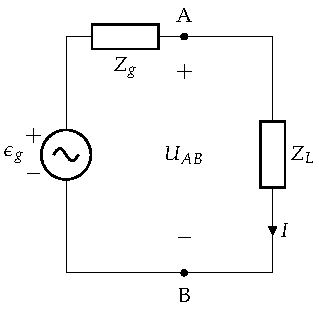
\includegraphics[height=0.45\textheight]{../figs/FuenteTensionRealACConCarga.pdf}
\end{center}

\begin{equation*}
  \left.
    \begin{matrix}
      \overline{Z}_L = \overline{Z}_g^*\\
      P_L = \frac{\epsilon^2_g}{|\overline{Z}_g + \overline{Z}_L|^2} \cdot R_L
    \end{matrix} \right\}\rightarrow
  \boxed{P_L = \frac{\epsilon^2_g}{4 R_g}}
\end{equation*}
\end{frame}

\begin{frame}[label={sec:org9bf794e}]{Máxima potencia de una fuente AC}
Si la impedancia de carga es resistiva pura, únicamente se puede cumplir la segunda condición del máximo, \(\diffp{P_L}{R_L} = 0\).
\begin{center}
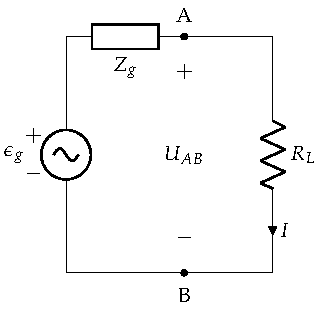
\includegraphics[height=0.4\textheight]{../figs/FuenteTensionRealACConCargaR.pdf}
\end{center}

En este caso, el resultado es:
\begin{align*}
      R_L &= |\overline{Z}_g| = \sqrt{R_g^2 + X_g^2}\\
      P_L &= \frac{\epsilon^2_g}{2(R_L + R_g)}
\end{align*}
\end{frame}

\section{Transformación y Asociación}
\label{sec:org7d03828}
\begin{frame}[label={sec:orga493ab6}]{Equivalencia de fuentes}
Sólo es posible establecer equivalencia entre \alert{fuentes reales}.
\begin{columns}
\begin{column}{0.33\columnwidth}
\begin{center}
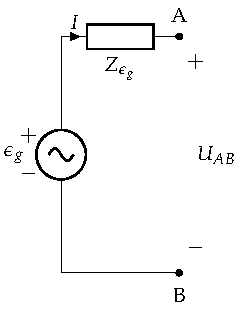
\includegraphics[height=0.5\textheight]{../figs/FuenteTensionReal.pdf}
\end{center}
\[
  \overline{U}_{AB} = \overline{\epsilon}_g - \overline{Z}_{\epsilon_g} \cdot \overline{I}
\]
\end{column}
\begin{column}{0.33\columnwidth}
\begin{align*}
  \overline{Z}_g &= \overline{Z}_{\epsilon_g} = \overline{Z}_{I_g}\\
  \overline{\epsilon}_g &= \overline{Z}_g \cdot \overline{I}_g\\
  \overline{I}_g &= \frac{\overline{\epsilon}_g}{\overline{Z}_g}
\end{align*}
\end{column}
\begin{column}{0.33\columnwidth}
\begin{center}
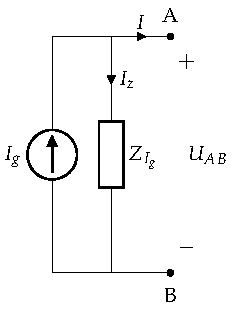
\includegraphics[height=0.5\textheight]{../figs/FuenteCorrienteReal.pdf}
\end{center}
\[
  \overline{I} = \overline{I}_g - \frac{\overline{U}_{AB}}{\overline{Z}_{I_g}}
\]
\end{column}
\end{columns}
\end{frame}


\begin{frame}[label={sec:org1dfe27a}]{Conexión en serie de generadores}
\begin{block}{Generadores de Tensión}
Pueden conectarse en serie sin restricción.

\begin{columns}
\begin{column}{0.5\columnwidth}
\begin{align*}
  \epsilon_t &= \sum_{i = 1}^N \epsilon_i\\
  R_{gt} &= \sum_{i = 1}^N R_{gi}\\ 
\end{align*}
\end{column}

\begin{column}{0.5\columnwidth}
\begin{align*}
  \overline{\epsilon}_t &= \sum_{i = 1}^N \overline{\epsilon}_i\\
  \overline{Z}_{gt} &= \sum_{i = 1}^N \overline{Z}_{gi}\\ 
\end{align*}
\end{column}
\end{columns}
\end{block}

\begin{block}{Generadores de Corriente}
\begin{itemize}
\item Ideal: todas las fuentes deben ser idénticas (valor y sentido).
\item Real:  sin restricción, transformación de fuentes para fuente equivalente.
\end{itemize}
\end{block}
\end{frame}


\begin{frame}[label={sec:orgb7e60a5}]{Conexión en paralelo de generadores}
\begin{block}{Generadores de Tensión}
\begin{itemize}
\item Ideal: todas las fuentes deben ser idénticas (valor y polaridad).
\item Real:  sin restricción, transformación de fuentes para fuente equivalente.
\end{itemize}
\end{block}


\begin{block}{Generadores de Corriente}
Pueden conectarse en paralelo sin restricción.
\begin{columns}
\begin{column}{0.5\columnwidth}
\begin{align*}
  I_{gT} &= \sum_{i = 1}^N I_{gi}\\
  G_{gT} &= \sum_{i = 1}^N G_{gi}\\ 
\end{align*}
\end{column}
\begin{column}{0.5\columnwidth}
\begin{align*}
  \overline{I}_{gt} &= \sum_{i = 1}^N \overline{I}_{gi}\\
  \overline{Y}_{gt} &= \sum_{i = 1}^N \overline{Y}_{gi}\\ 
\end{align*}
\end{column}
\end{columns}
\end{block}
\end{frame}


\begin{frame}[label={sec:org1ae0360}]{Fuentes dominantes}
Una fuente de tensión es dominante sobre las ramas conectadas en paralelo.
\begin{center}
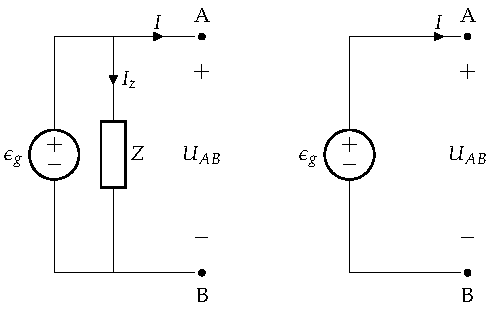
\includegraphics[height=0.8\textheight]{../figs/FuenteTensionDominante.pdf}
\end{center}
\end{frame}

\begin{frame}[label={sec:org37e3885}]{Fuentes dominantes}
Una fuente de corriente es dominante sobre los elementos conectados en serie.
\begin{center}
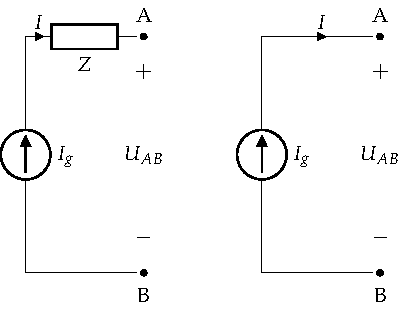
\includegraphics[height=0.8\textheight]{../figs/FuenteCorrienteDominante.pdf}
\end{center}
\end{frame}

\begin{frame}[label={sec:orgc899f67}]{Modificación de la geometría de un circuito}
\begin{columns}
\begin{column}{0.5\columnwidth}
\begin{center}
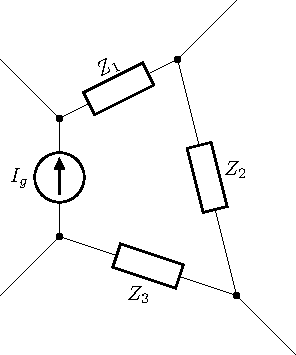
\includegraphics[height=0.8\textheight]{../figs/ModificacionGeometria_FuenteCorriente.pdf}
\end{center}
\end{column}

\begin{column}{0.5\columnwidth}
\begin{center}
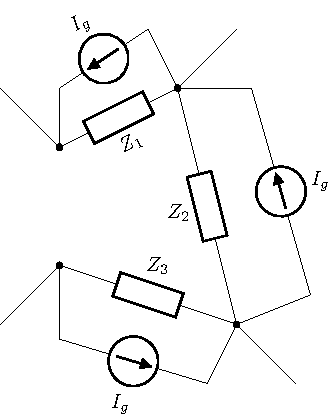
\includegraphics[height=0.8\textheight]{../figs/ModificacionGeometria_FuenteCorriente2.pdf}
\end{center}
\end{column}
\end{columns}
\end{frame}

\begin{frame}[label={sec:orgd6d6ea1}]{Modificación de la geometría de un circuito}
\begin{columns}
\begin{column}{0.5\columnwidth}
\begin{center}
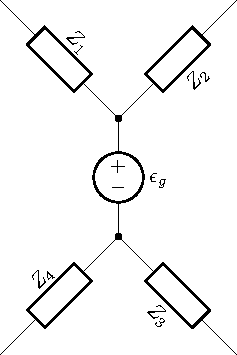
\includegraphics[height=0.8\textheight]{../figs/ModificacionGeometria_FuenteTension.pdf}
\end{center}
\end{column}

\begin{column}{0.5\columnwidth}
\begin{center}
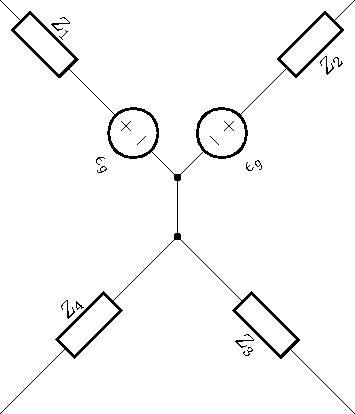
\includegraphics[height=0.8\textheight]{../figs/ModificacionGeometria_FuenteTension2.pdf}
\end{center}
\end{column}
\end{columns}
\end{frame}

\begin{frame}[label={sec:org806a3c7}]{Modificación de la geometría de un circuito}
\begin{columns}
\begin{column}{0.5\columnwidth}
\begin{center}
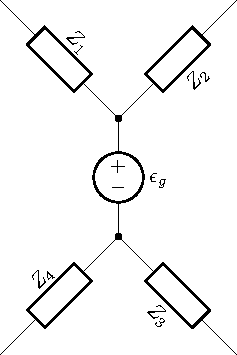
\includegraphics[height=0.8\textheight]{../figs/ModificacionGeometria_FuenteTension.pdf}
\end{center}
\end{column}

\begin{column}{0.5\columnwidth}
\begin{center}
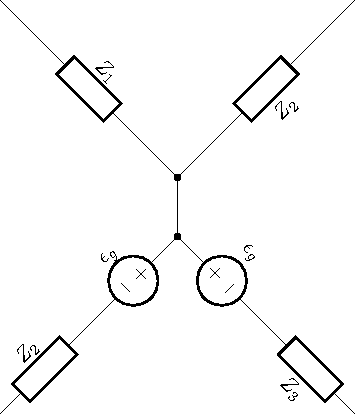
\includegraphics[height=0.8\textheight]{../figs/ModificacionGeometria_FuenteTension3.pdf}
\end{center}
\end{column}
\end{columns}
\end{frame}
\end{document}